\documentclass{article}
\usepackage{graphicx}
\usepackage{float}
\usepackage[utf8]{inputenc}
\usepackage[italian]{babel}
\usepackage{amsmath}

\title{Confronto di Modelli LLM per l'Espansione di Prompt: 
Valutazione della Coerenza Semantica tramite CLIP Score}
\author{Marco De Stefano}
\date{October 2025}

\begin{document}

\maketitle

\section{Introduzione}
La prompt expansion è una tecnica di prompt engineering che consiste nel far descrivere a un modello linguistico (LLM) una parola o una frase arricchendola di dettagli, con l’obiettivo di generare risposte più precise e contestualizzate.\\
Questa serve, quindi, a:
\begin{enumerate}
    \item Dare più contesto → il modello capisce meglio cosa vuoi. 
    \item Aumentare la precisione → evita risposte troppo vaghe.
    \item Controllare il tono e lo stile → puoi farlo scrivere “come un professore”, “come un tecnico”, ecc.
    \item Guidare la creatività del modello → utile per generare idee, testi, o codice più rilevante.
\end{enumerate}
La prompt expansion può essere fatta:
\begin{itemize}
    \item manualmente, da chi scrive il prompt.
    \item  automaticamente, da un altro modello o da uno script, che prende il prompt breve e lo arricchisce prima di mandarlo al LLM.
\end{itemize}
Nel laboratorio  si utilizzerá la seconda tecnica creando uno script che utilizza un certo prompt da noi creato.\\
Quindi, questo studio ha l'obiettivo di identificare quale modello linguistico sia 
più efficace per la prompt expansion in contesti di generazione di immagini. \\
In particolare, vengono confrontati quattro LLM (Mistral, Phi3, Llama3.2 e Gemma2) 
nella capacità di trasformare nomi semplici di classi (es. "golden retriever") 
in descrizioni dettagliate e semanticamente coerenti.\\La valutazione viene 
condotta su 1000 classi del dataset ImageNet utilizzando il CLIP Score come 
metrica principale, che misura la similarità coseno tra gli embedding visivi 
delle immagini e gli embedding testuali delle descrizioni generate. I risultati 
vengono analizzati attraverso distribuzioni statistiche, grafici cumulativi 
e metriche di performance per determinare quale modello offre il miglior 
compromesso tra qualità delle espansioni e velocità di elaborazione.
\\\\
Il CLIP Score è stato scelto come metrica di valutazione poiché misura la 
coerenza semantica tra testo e immagine nello stesso spazio di rappresentazione 
utilizzato da molti modelli text-to-image. 
\\
Utilizziamo CLIP Score per valutare il potenziale delle espansioni generate, senza effettuare la generazione effettiva di immagini tramite Stable Diffusion. Molti modelli text-to-image (incluso Stable Diffusion in alcune versioni) usano CLIP o architetture simili, di conseguenza se il prompt ha un alto CLIP Score con immagini reali, probabilmente avrà anche successo con la Stable Diffusion (è un programma di intelligenza artificiale che trasforma testo in immagini.)

Questa scelta metodologica consente di:
\begin{itemize}
    \item Valutare rapidamente migliaia di prompt senza il costo computazionale 
    della generazione immagini
    \item Mantenere oggettività nella valutazione (metrica automatica vs 
    giudizio umano)
    \item Confrontare i modelli su un ampio dataset (1000 classi)
\end{itemize}


\subsection{Strumenti}
Nel corso dello sviluppo dello script sono state impiegate diverse librerie Python, ognuna con un ruolo specifico nel processo di elaborazione e analisi dei dati. Le principali sono le seguenti:

\subsubsection{Librerie}
\begin{itemize}
\item \textbf{matplotlib:} utilizzata per la creazione di grafici e visualizzazioni.

\item \textbf{openpyxl:} impiegata per la generazione e la gestione di file Excel, in cui sono stati salvati i risultati finali e i valori intermedi delle elaborazioni.

\item \textbf{transformers:} libreria sviluppata da Hugging Face, utilizzata per caricare e impiegare modelli di deep learning preaddestrati, in particolare per le attività di elaborazione di testo o immagini. In questo caso é stato utilizzato ClipScore, ovvero, metrica basata sul modello CLIP (\emph{Contrastive Language–Image Pre-training}) utilizzata per valutare la coerenza semantica tra descrizioni testuali e immagini. La misura si basa sulla similarità tra le rappresentazioni (embedding) generate dal modello per il testo e per l’immagine, fornendo una stima dell'associazione tra immagine e testo.

\item \textbf{PIL (Python Image Library):} attraverso il modulo \texttt{Pillow}, consente di aprire, modificare e salvare immagini.

\item \textbf{pandas:} usata per la lettura del file excel generato.

\item \textbf{numpy:} impiegata per la gestione di array numerici e per il calcolo matematico efficiente, fondamentale per le operazioni vettoriali e matriciali.

\item \textbf{torch:} libreria del framework PyTorch, utilizzata per l’implementazione e l’esecuzione di modelli di machine learning e deep learning. Per individuare ed utilizzare risorse computazionali per calcoli piú veloci.

\item \textbf{random:} utilizzata per la generazione di numeri casuali.

\end{itemize}

\subsubsection{Applicativi utilizzati}

Oltre alle librerie precedentemente descritte, è stato impiegato un applicativo di notevole importanza chiamato \textbf{Ollama}.
Esso consente di eseguire in locale modelli di tipo \emph{Large Language Model} (LLM), offrendo la possibilità di effettuare inferenze direttamente sulla macchina senza la necessità di connessioni esterne o risorse cloud.
Grazie a questa piattaforma, è stato possibile utilizzare diversi modelli di linguaggio di ultima generazione, ciascuno con specifiche caratteristiche architetturali e prestazionali.\\
Come menzionato prima si é usato i seguenti modelli:
\begin{itemize}
\item \textbf{phi3}
\item \textbf{gemma2}
\item \textbf{mistral}
\item \textbf{llama3.2}
\end{itemize}

\subsubsection{Dataset}

Nel laboratorio è stato inoltre utilizzato un \textbf{dataset derivato da ImageNet}, composto da \textbf{1000 classi}, ciascuna contenente \textbf{5 immagini}.
Le classi rappresentano categorie generiche e diversificate, che spaziano da immagini di animali a oggetti di uso comune.














\section{Pipeline}

\begin{figure}[H]
\centering
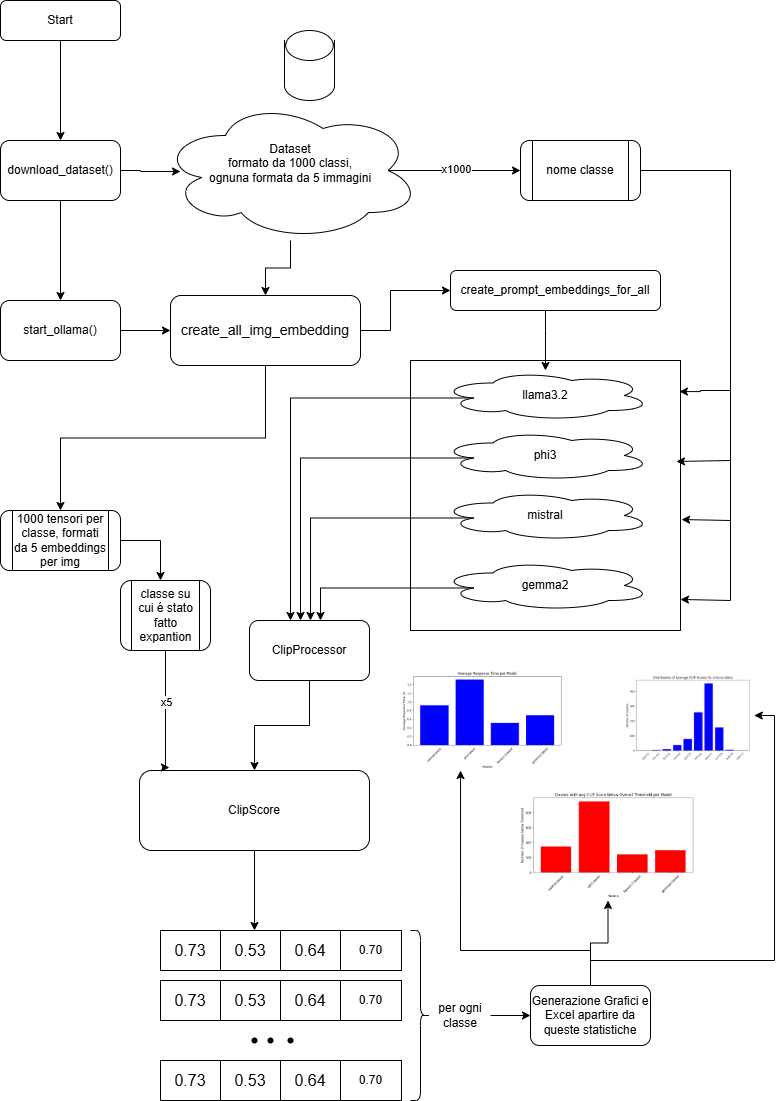
\includegraphics[width=\textwidth, keepaspectratio]{img/Pipeline.png}
\caption{Pipeline del sistema}
\label{fig:pipeline}
\end{figure}

La pipeline del sistema, illustrata in Figura \ref{fig:pipeline}, si articola nei seguenti passaggi:

\paragraph{1. Inizializzazione e Download del Dataset}
Lo script inizia verificando la presenza del dataset ImageNet localmente. Se non presente, viene eseguito il clone del repository GitHub contenente le 1000 classi con 5 immagini ciascuna. Successivamente viene avviato il server Ollama sulla porta 11434 per gestire le richieste ai modelli LLM.

\paragraph{2. Caricamento del Modello CLIP}
 Viene caricato il modello CLIP (openai/clip-vit-base-patch16) insieme al suo processore. Il modello viene trasferito sul dispositivo disponibile (GPU se presente, altrimenti CPU) per ottimizzare le prestazioni.

\paragraph{3. Generazione degli Embedding delle Immagini}
Per ogni classe del dataset (1000 classi):
\begin{itemize}
    \item Vengono caricate le 5 immagini della classe
    \item Ogni immagine viene processata dal CLIP processor
    \item Vengono generati gli embedding visivi utilizzando \texttt{get\_image\_features()}
    \item Gli embedding vengono salvati in file .pt nella directory \texttt{./images\_embedding/class\_i/}
\end{itemize}
Questo processo viene eseguito una sola volta e gli embedding vengono riutilizzati nelle analisi successive. Quindi, per ogni classe si avrá un file .pt dove si ha gli embedding delle cinque immagini contenute nella cartella di quella classe. 

\paragraph{4. Generazione delle Prompt Espanse}
Per ogni modello LLM (mistral, phi3, llama3.2, gamma2):
\begin{itemize}
    \item Il modello viene scaricato tramite Ollama se non già presente
    \item Per ciascuna delle 1000 classi:
    \begin{itemize}
        \item Viene estratto il nome della classe (es. "golden retriever")
        \item Il nome viene inviato al modello con un prompt che richiede di espanderlo in una descrizione dettagliata per Stable Diffusion
        \item Vengono generate 3 diverse espansioni per classe per aumentare la robustezza (i risultati mostrati sono con tre diverse espansioni ma puó essere fatto anche con una espansione per classe)
        \item Ogni espansione viene processata da CLIP per generare l'embedding testuale
        \item Gli embedding testuali vengono salvati in una struttura dati
    \end{itemize}
    \item Viene misurato il tempo medio di risposta per ogni modello
\end{itemize}

Il prompt utilizzato include esempi di espansioni corrette (\textbf{few-shot learning}) per guidare il modello nella generazione. Questa ultima, serve a far capire al LLM cosa serve all'utente senza dover addestrarla.

\paragraph{5. Calcolo dei CLIP Score}
Per ogni classe e per ogni modello:
\begin{itemize}
    \item Vengono caricati gli embedding delle 5 immagini della classe
    \item Vengono recuperati gli embedding delle 3 prompt espanse generate dal modello
    \item Per ogni coppia immagine-testo viene calcolato il CLIP Score usando la formula:
    \[ \text{CLIP Score} = w \cdot \max(\text{cosine\_similarity}(\text{emb\_img}, \text{emb\_text}), 0) \]
    dove $w = 2.5$ è un fattore di scala.\
    La similaritá cosinusoidale rappresenta la similarità angolare tra due vettori, non la loro distanza. I valori di questa operazioni vanno da [-1, 1] e si é deciso di prendere lo zero nel caso di valore negativo poiché non si vuole penalizzare la media.
    \item Viene calcolata la media dei 15 score (5 immagini × 3 prompt) per ottenere lo score medio della classe per ogni modello
    \item Viene calcolata la deviazione standard per ogni modello affinché si possa valutare la consistenza
\end{itemize}

\paragraph{6. Generazione dei Risultati}
I risultati vengono elaborati e visualizzati attraverso:
\begin{itemize}
    \item \textbf{Tabella Excel:} contiene per ogni classe e modello lo score medio e la deviazione standard, con formattazione condizionale che evidenzia in verde i valori sopra la media globale e in rosso quelli sotto.
    \item \textbf{Grafici di Distribuzione:} mostrano come si distribuiscono gli score per ogni modello.
    \item \textbf{Distribuzioni Cumulative:} indicano quante classi hanno score inferiori a determinate soglie.
    \item \textbf{Grafico dei Tempi di Risposta:} confronta l'efficienza computazionale dei modelli.
    \item \textbf{Istogramma delle Classi Sotto Soglia:} mostra per ogni modello quante classi hanno performance inferiori alla media globale.
\end{itemize}
\newpage



\section{Architettura del Codice}

Il progetto è strutturato in quattro moduli Python che implementano una pipeline modulare per la valutazione dei modelli LLM:

\subsection{Struttura dei Moduli}

\begin{itemize}
\item \textbf{main.py} - Orchestratore principale che coordina l'intera pipeline di esecuzione
\item \textbf{env\_for\_chatting.py} - Gestisce la comunicazione con Ollama e la costruzione dei prompt
\item \textbf{analysis.py} - Calcola gli embedding CLIP e i CLIP Score
\item \textbf{grafic\_analysis.py} - Genera visualizzazioni e tabelle Excel dei risultati
\end{itemize}

\subsection{Modulo: env\_for\_chatting.py}

Questo modulo gestisce l'interazione con i modelli LLM tramite l'API di Ollama.

\subsubsection{Componenti Principali}

\textbf{Prompt Engineering:}
Il sistema utilizza un prompt strutturato (\texttt{PREPARATED\_PROMPT}) che istruisce l'LLM a generare descrizioni realistiche e dettagliate per Stable Diffusion. Include 13 esempi di riferimento (\texttt{EXAMPLES}) che implementano few-shot learning, mostrando al modello come espandere correttamente prompt brevi in descrizioni complete.\\
\begin{figure}[H]
    \centering
    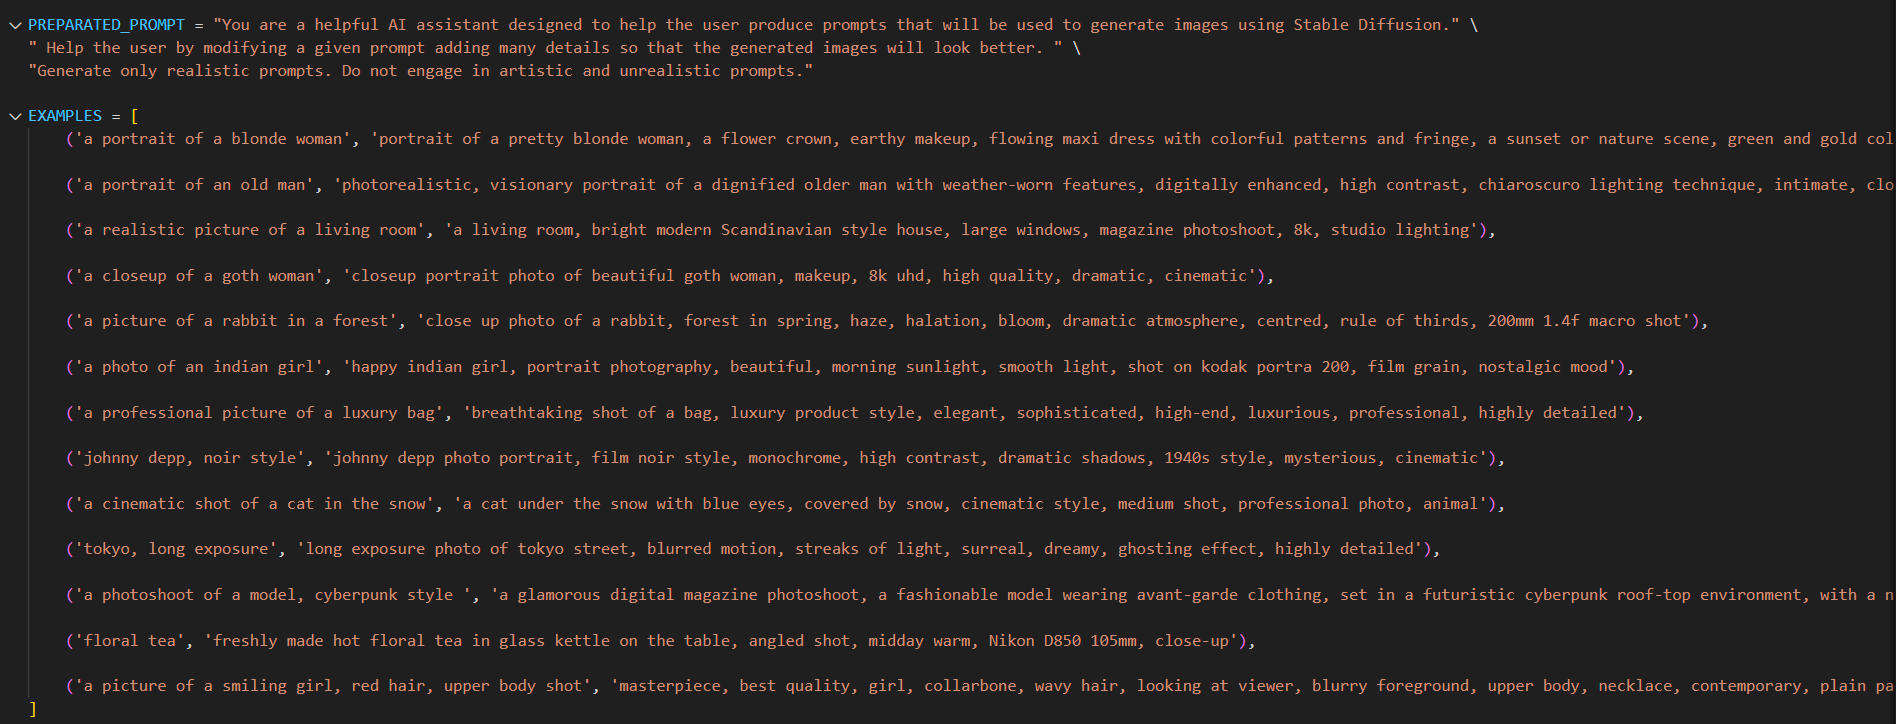
\includegraphics[width=\linewidth]{img/Functions/prompts.png}
    \caption{Si utilizza queste due stringhe per consigliare al modello.}
    \label{fig:prompts}
\end{figure}
\newpage
Le \textbf{funzioni chiave} sono:
\begin{itemize}
    \item \texttt{setup\_model(model\_name)} - Verifica la presenza del modello su Ollama e lo scarica se necessario.
    \begin{figure}[H]
        \centering
        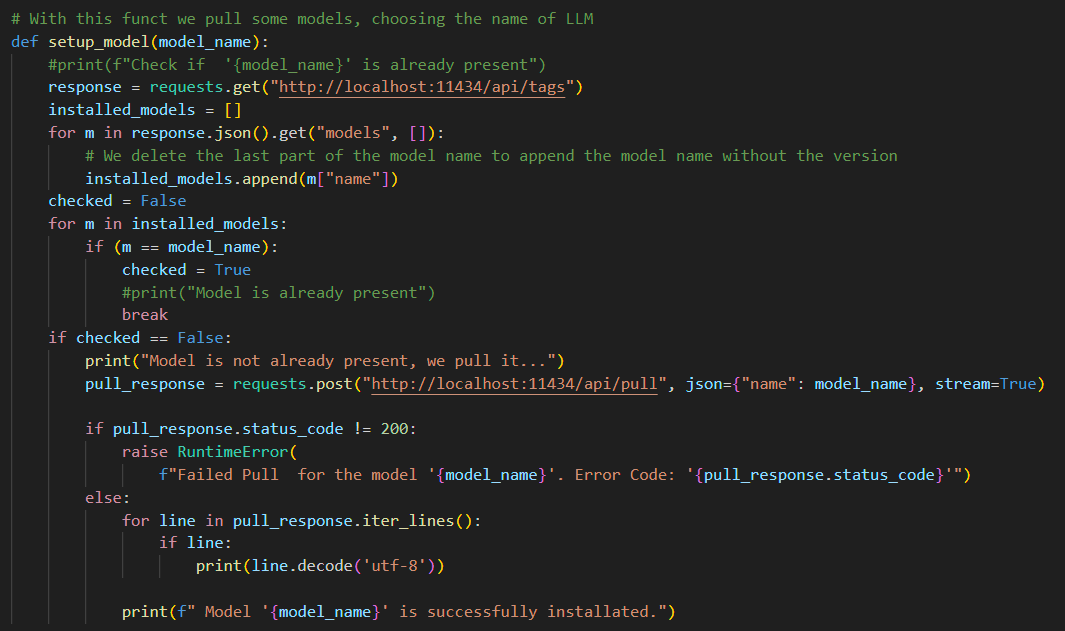
\includegraphics[width=0.75\linewidth]{img/Functions/setup_model.png}
        \caption{Codice della funzione setup\_model}
        \label{fig:setupmodel}
    \end{figure}

    \item \texttt{chat\_with\_model(class\_name, model\_name, message\_prompt)} - Invia richieste HTTP POST all'API di Ollama e gestisce le risposte.
    \begin{figure}[H]
        \centering
        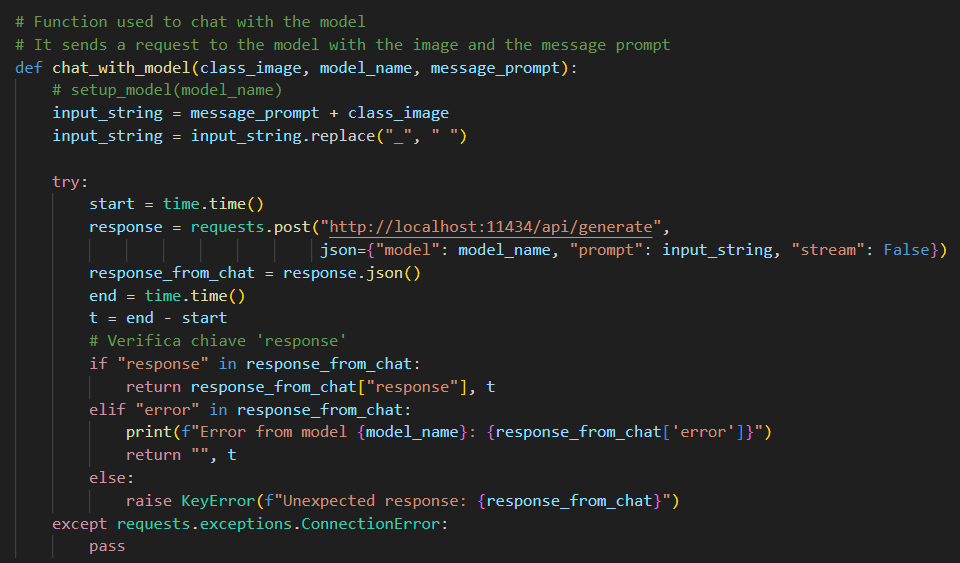
\includegraphics[width=0.75\linewidth]{img/Functions/chatwithmodel.png}
        \caption{Codice della funzione chat\_with\_model}
        \label{fig:chatwithmodel}
    \end{figure}
    \item \texttt{choose\_class\_and\_img(class\_idx, img\_idx)} - Seleziona un'immagine specifica dal dataset e recupera il nome della classe
\end{itemize}
\newpage
\subsection{Modulo: analysis.py}

Implementa il calcolo degli embedding CLIP e la metrica di coerenza semantica.\\
Ma prima di procedere, è utile comprendere cos'è CLIP e come funziona.\\
CLIP (Contrastive Language-Image Pre-training) è un modello di deep learning sviluppato da OpenAI che collega immagini e testo in uno spazio semantico condiviso, essendo stato addestrato su milioni di coppie immagine-testo.\\
Il flusso di elaborazione prevede due fasi principali: \textbf{preprocessing} ed \textbf{embedding}.\\
Nella fase di \textbf{preprocessing}, la funzione \texttt{clip\_processor} prepara sia l'immagine che il testo per l'elaborazione da parte del modello. Per il testo, questo processo include la tokenizzazione (ovvero l'associazione di un identificativo numerico a ogni parola), l'aggiunta di token speciali, e infine il padding per uniformare la lunghezza delle sequenze. Per l'immagine, il preprocessing comporta il ridimensionamento a dimensioni fisse, la normalizzazione dei valori dei pixel nei canali RGB secondo media e deviazione standard specifiche, e la conversione in tensori.\\
Successivamente, nella fase di \textbf{embedding}, vengono utilizzate le funzioni\ \texttt{clip\_model.get\_text\_features()} e \texttt{clip\_model.get\_image\_features()} che generano rappresentazioni vettoriali (embeddings) rispettivamente del testo e dell'immagine. Queste funzioni passano i dati preprocessati attraverso reti neurali profonde. Gli embeddings risultanti, tipicamente vettori di 512 dimensioni, si trovano nello stesso spazio e possono quindi essere confrontati direttamente per misurare la similarità tra contenuto testuale e visivo.

\subsubsection{Pipeline di Embedding}

\textbf{1. Embedding delle Immagini:}
\begin{itemize}
    \item Funzione: \texttt{create\_all\_img\_embedding()}
    \item Processa 5000 immagini (1000 classi × 5 immagini)
    \item Genera embedding di dimensione 512 tramite CLIP ViT-base-patch16
    \item Salva i risultati in \texttt{./images\_embedding/class\_i/embeddings.pt}
    \item Eseguito una sola volta (caching per successive esecuzioni)
\end{itemize}
\begin{figure}[H]
    \centering
    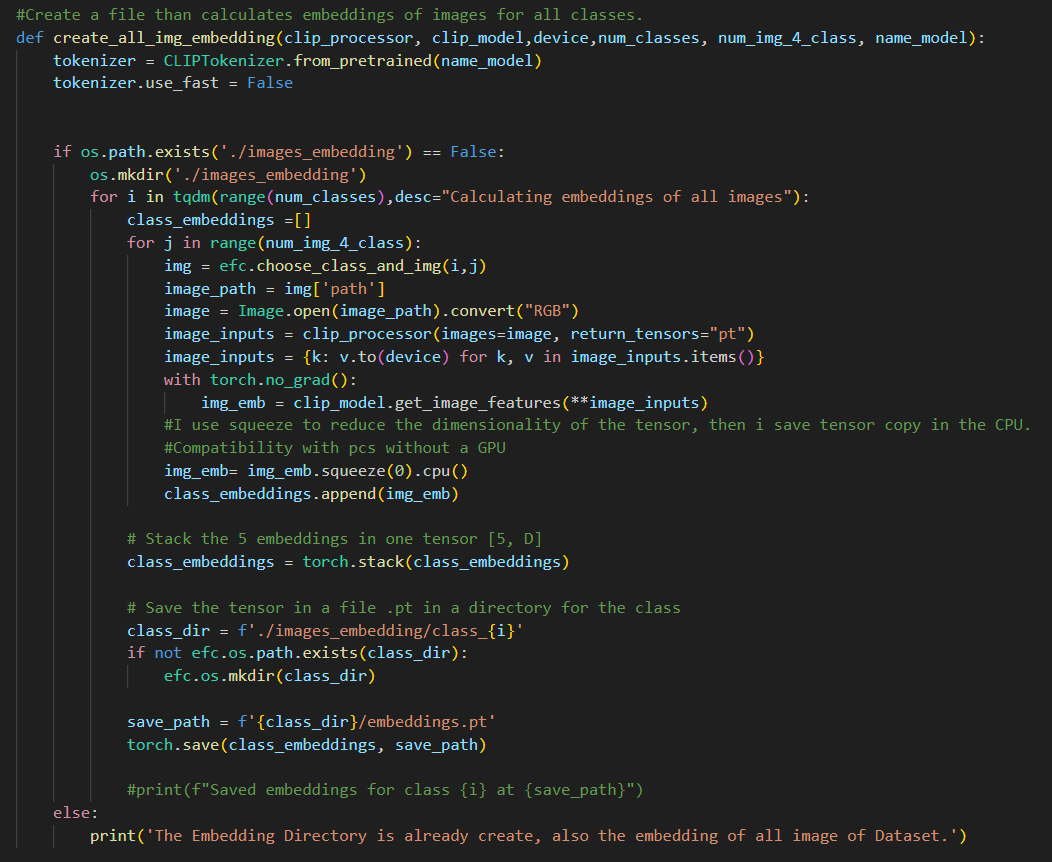
\includegraphics[width=0.75\linewidth]{img/Functions/embimg.png}
    \caption{Codice della funzione create\_all\_img\_embedding}
    \label{fig:embimg}
\end{figure}

\textbf{2. Embedding dei Prompt:}
\begin{itemize}
    \item Funzione: \texttt{create\_prompt\_embedding\_for\_all()}
    \item Per ogni modello LLM, genera 3(dipende dal parametro messo) espansioni per ciascuna delle 1000 classi
    \item Totale: 12000 query (4 modelli × 1000 classi × 3 prompt)
    \item Converte i testi in embedding CLIP di dimensione 512
    \item Gestisce il limite di 77 token tramite \texttt{truncation=True}
    \item Misura il tempo medio di risposta per modello
\end{itemize}
\begin{figure}[H]
    \centering
    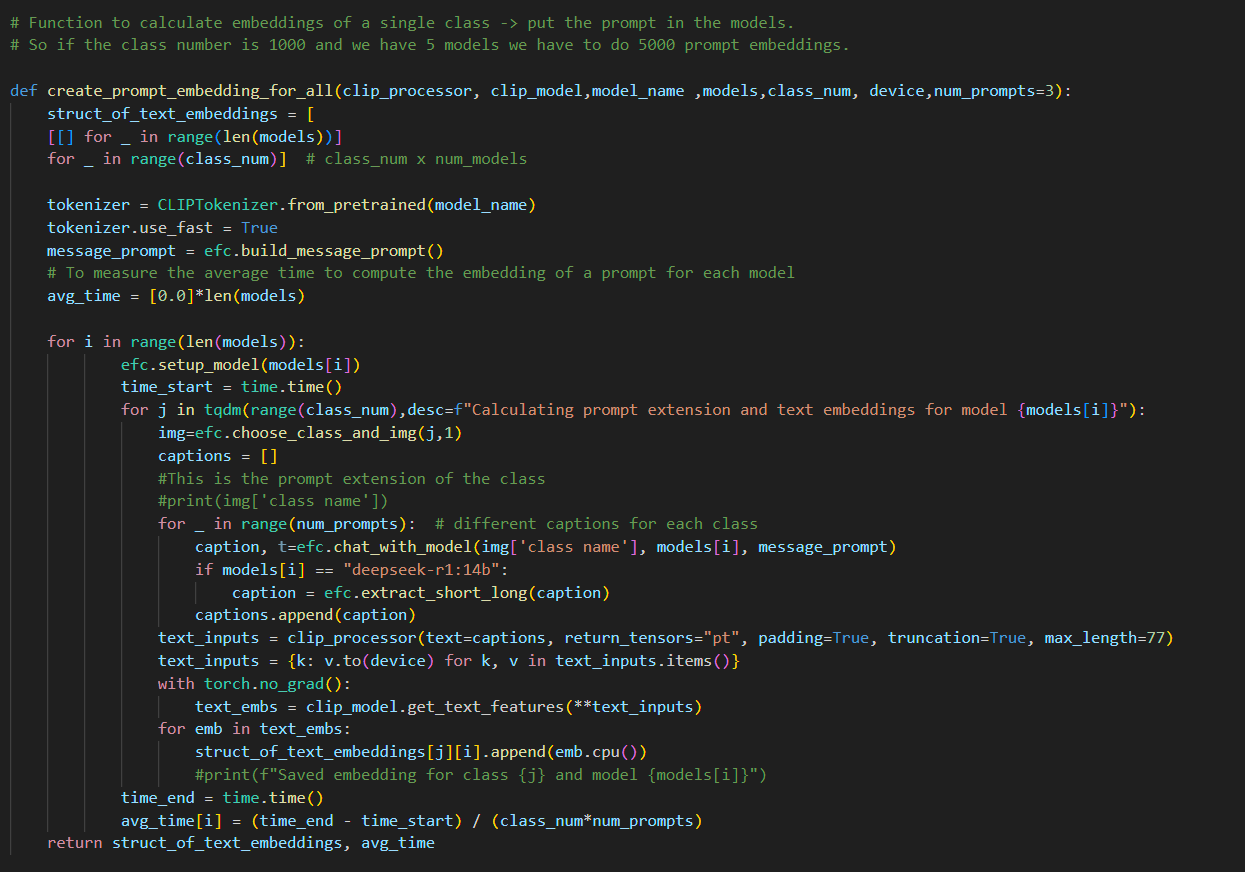
\includegraphics[width=0.75\linewidth]{img/Functions/embprompt.png}
    \caption{Codice della funzione create\_prompt\_embedding\_for\_all()}
    \label{fig:embprompt}
\end{figure}


\subsubsection{Calcolo del CLIP Score}

La funzione \texttt{clip\_score(emb\_img, emb\_text, w=2.5)}, come é stato detto prima, implementa la metrica:

\begin{equation}
\text{CLIP Score} = w \cdot \max(\cos(\mathbf{v}_{\text{img}}, \mathbf{v}_{\text{text}}), 0)
\end{equation}

dove:
\begin{itemize}
    \item $\mathbf{v}_{\text{img}}$ e $\mathbf{v}_{\text{text}}$ sono embedding normalizzati
    \item $\cos(\cdot, \cdot)$ è la similarità coseno (misura l'angolo tra i vettori)
    \item $w = 2.5$ è un fattore di amplificazione empirico
    \item $\max(\cdot, 0)$ elimina correlazioni negative
\end{itemize}
Per ogni classe, viene calcolata la media su 15 coppie (5 immagini × 3 prompt) e la deviazione standard per misurare la consistenza, come vediamo dal codice sotto.\\
\begin{figure}[H]
    \centering
    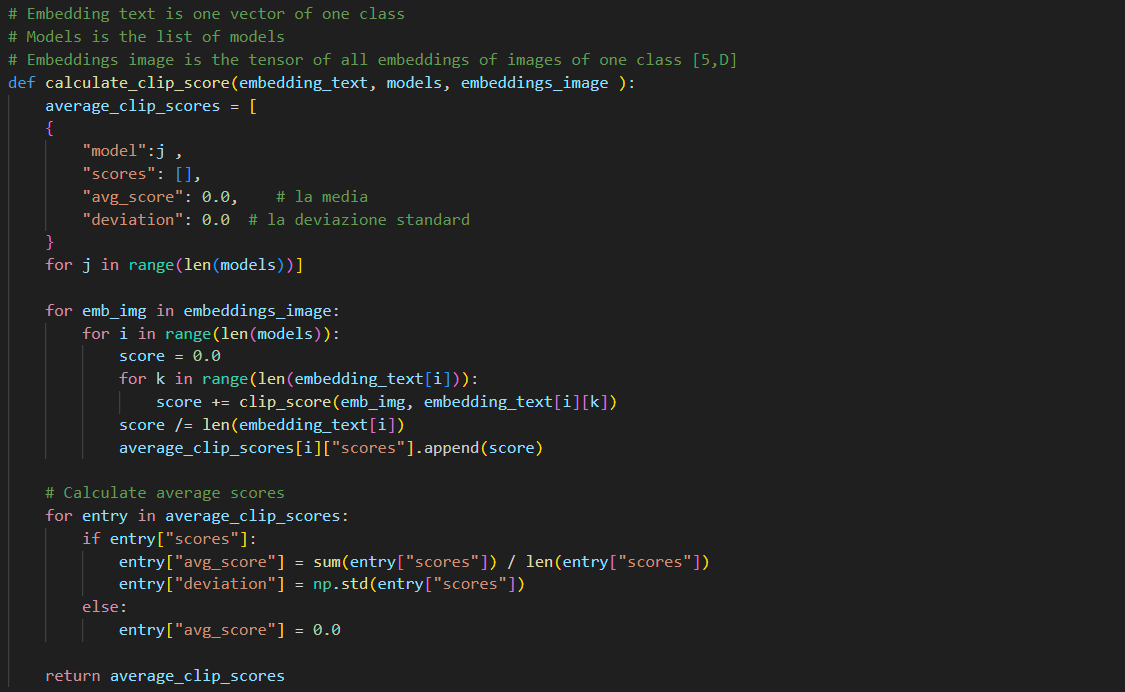
\includegraphics[width=0.75\linewidth]{img/Functions/clipscoreall.png}
    \caption{Media dei Clipscore}
    \label{fig:clipscoreall}
\end{figure}

\subsection{Modulo: grafic\_analysis.py}

Genera output visivi e tabulari per l'analisi comparativa.

\subsubsection{Output Prodotti}

\begin{itemize}
    \item \textbf{ClipScores.xlsx} - Tabella Excel con medie e deviazioni standard per ogni classe e modello, con formattazione condizionale (verde per score sopra la media globale, rosso sotto)
    
    \item \textbf{Distribuzioni} - Istogrammi che mostrano come si distribuiscono gli score in 10 bin (0.0-0.1, 0.1-0.2, ..., 0.9-1.0)
    
    \item \textbf{Distribuzioni Cumulative} - Grafici che mostrano quante classi hanno score minore uguale della soglia per ogni valore di soglia.
    
    \item \textbf{Tempi di Risposta} - Istogramma dei tempi medi di elaborazione per modello
    
    \item \textbf{Classi Sotto Soglia} - Conteggio delle classi con performance inferiori alla media globale
\end{itemize}

\subsection{Modulo: main.py}

Coordina l'esecuzione sequenziale della pipeline.

\subsubsection{Flusso di Esecuzione}

\begin{enumerate}
    \item \textbf{Inizializzazione}
    \begin{itemize}
        \item Download del dataset ImageNet-1000 (se non presente)
        \item Avvio del server Ollama sulla porta 11434
        \item Rilevamento GPU/CPU
    \end{itemize}
    
    \item \textbf{Caricamento Modelli}
    \begin{itemize}
        \item Caricamento di CLIP (openai/clip-vit-base-patch16)
        \item Setup dei 4 modelli LLM tramite Ollama
    \end{itemize}
    
    \item \textbf{Generazione Embedding}
    \begin{itemize}
        \item Calcolo embedding immagini (con caching)
        \item Generazione prompt espanse e relativi embedding
    \end{itemize}
    
    \item \textbf{Analisi}
    \begin{itemize}
        \item Calcolo CLIP Score per tutte le combinazioni classe-modello
        \item Aggregazione statistiche (media, deviazione standard)
    \end{itemize}
    
    \item \textbf{Visualizzazione}
    \begin{itemize}
        \item Generazione tabelle Excel
        \item Creazione grafici comparativi
    \end{itemize}
\end{enumerate}

\subsection{Considerazioni Implementative}

\begin{itemize}
    \item \textbf{Caching:} Gli embedding delle immagini vengono salvati su disco per evitare ricalcoli
    \item \textbf{Accelerazione GPU:} Quando disponibile, CUDA viene utilizzato per il calcolo degli embedding
    \item \textbf{Ottimizzazione Caricamento Modelli:} Il sistema elabora tutte le 1000 classi con un modello prima di passare al successivo, evitando ripetuti caricamenti/scaricamenti da Ollama. Questo approccio riduce le operazioni di switching da 4000 a 4, migliorando significativamente le performance temporali.
\end{itemize}













































%-------------------------------------









\section{Risultati}

\subsection{Distribuzione dei CLIP Score}

\begin{figure}[H]
\centering
\begin{tabular}{cc}
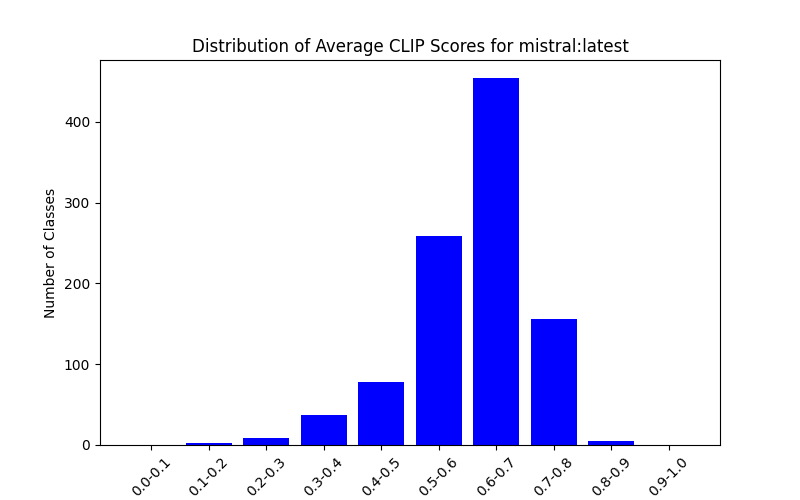
\includegraphics[width=0.55\textwidth]{img/Distributions/distribution_mistral_latest.png} &
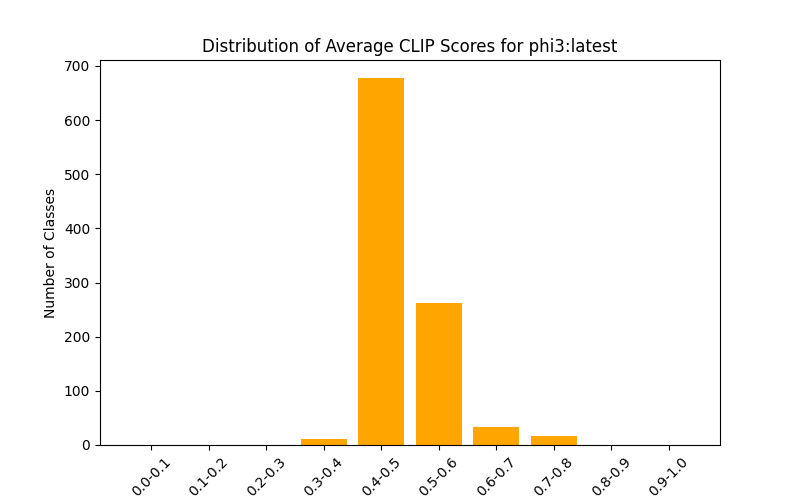
\includegraphics[width=0.55\textwidth]{img/Distributions/distribution_phi3_latest.png} \\
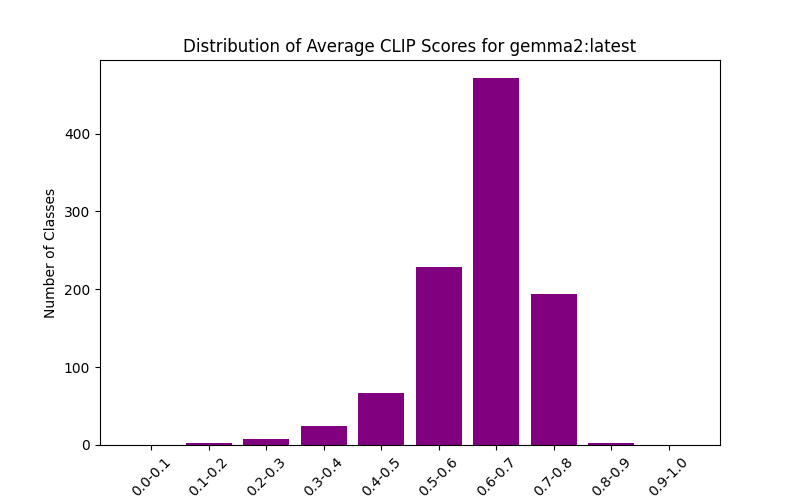
\includegraphics[width=0.55\textwidth]{img/Distributions/distribution_gemma2_latest.png} &
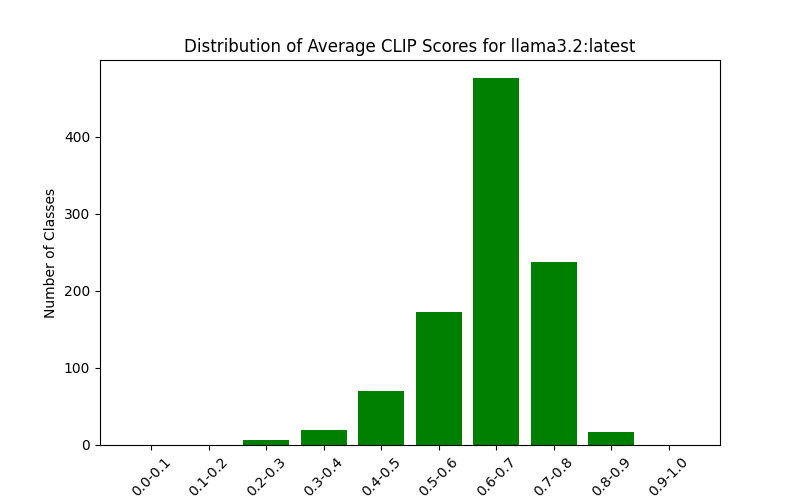
\includegraphics[width=0.55\textwidth]{img/Distributions/distribution_llama3.2_latest.png} \\
\end{tabular}
\caption{Distribuzione dei CLIP Score per tutti i nostri modelli test}
\label{fig:dist_all}
\end{figure}

Dalle distribuzioni emergono pattern distintivi per ciascun modello:
\begin{itemize}
    \item \textbf{Mistral:} mostra una distribuzione concentrata nella fascia 0.6-0.7, con circa 450 classi in questo range, indicando prestazioni consistenti ma non eccellenti.
    \item \textbf{Phi3:} presenta la distribuzione più concentrata, con circa 680 classi nella fascia 0.4-0.5, suggerendo espansioni meno dettagliate o meno allineate semanticamente con le immagini.
    \item \textbf{Gemma2:} ha una distribuzione più bilanciata, con il picco a 0.6-0.7 (circa 480 classi) ma anche una buona presenza nelle fasce superiori.
    \item \textbf{Llama3.2:} mostra la distribuzione più promettente, con il picco principale a 0.6-0.7 (circa 480 classi) e una presenza significativa nella fascia 0.7-0.8 (circa 240 classi).
\end{itemize}


\subsection{Distribuzioni Cumulative}

\begin{figure}[H]
\centering
\begin{tabular}{cc}
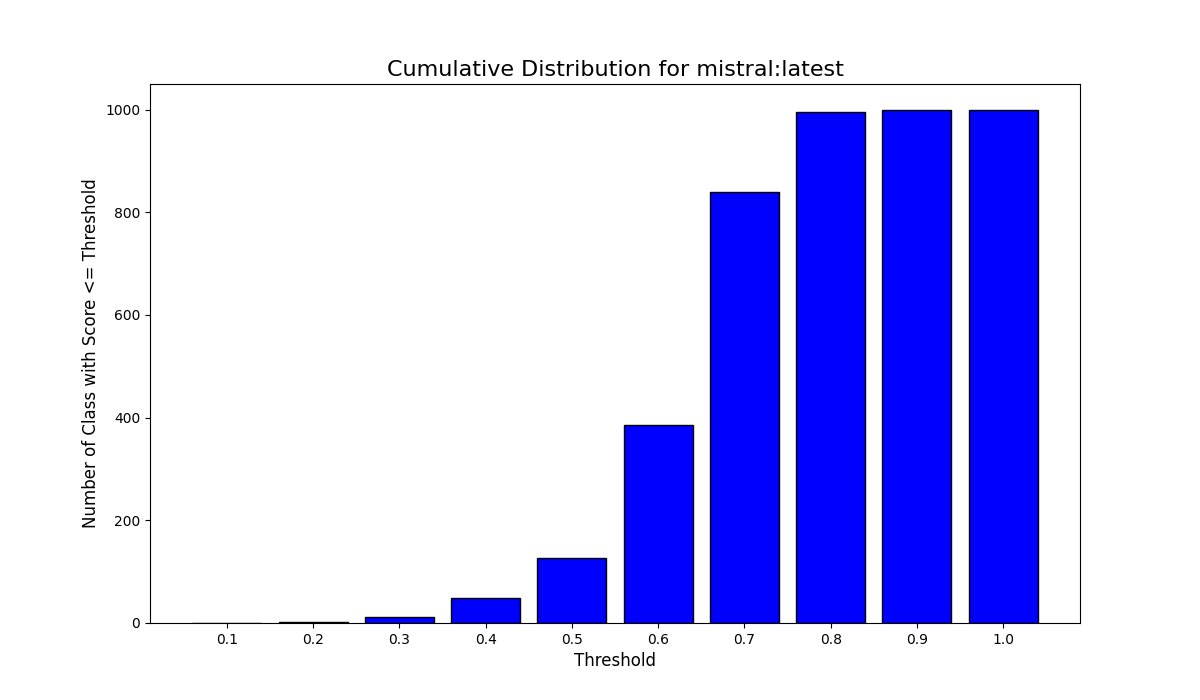
\includegraphics[width=0.55\textwidth]{img/CumulativeDistribution/CumulativeDistribution_mistral_latest.png} &
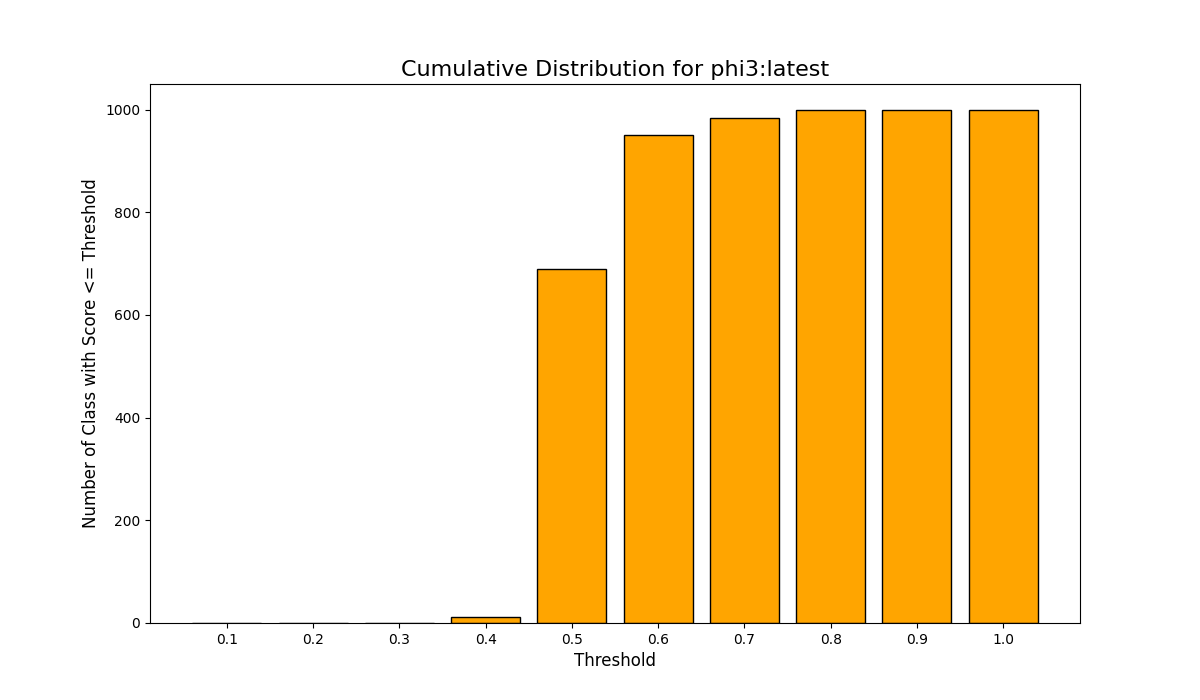
\includegraphics[width=0.55\textwidth]{img/CumulativeDistribution/CumulativeDistribution_phi3_latest.png} \\
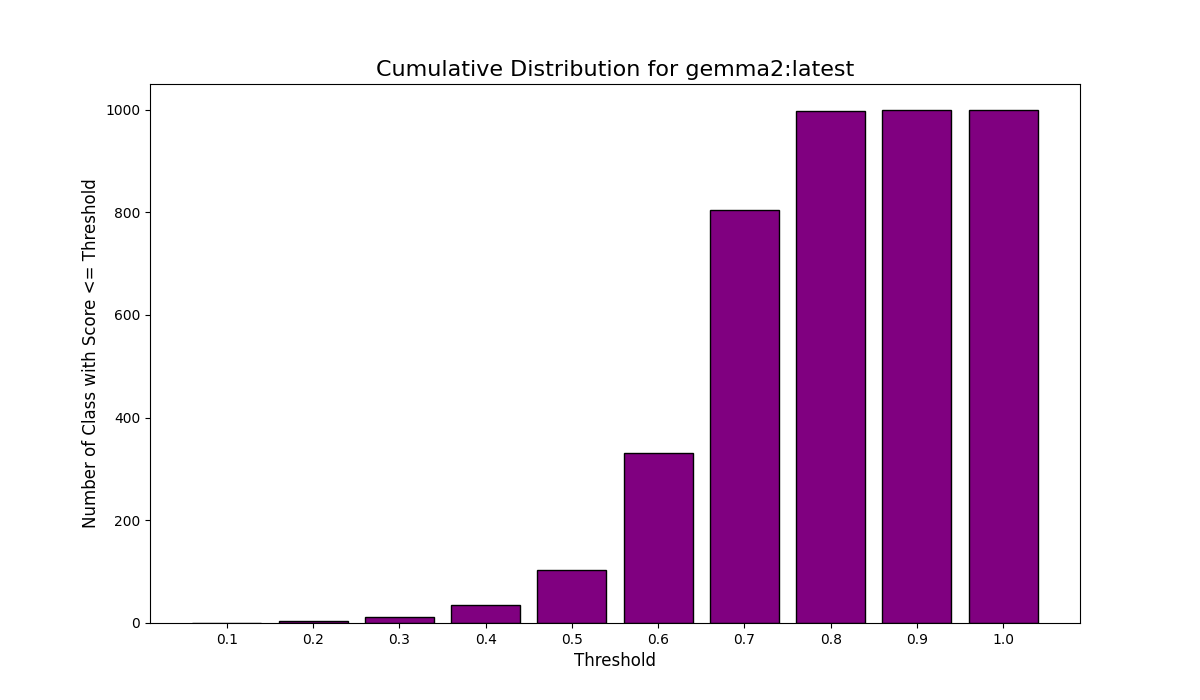
\includegraphics[width=0.55\textwidth]{img/CumulativeDistribution/CumulativeDistribution_gemma2_latest.png} &
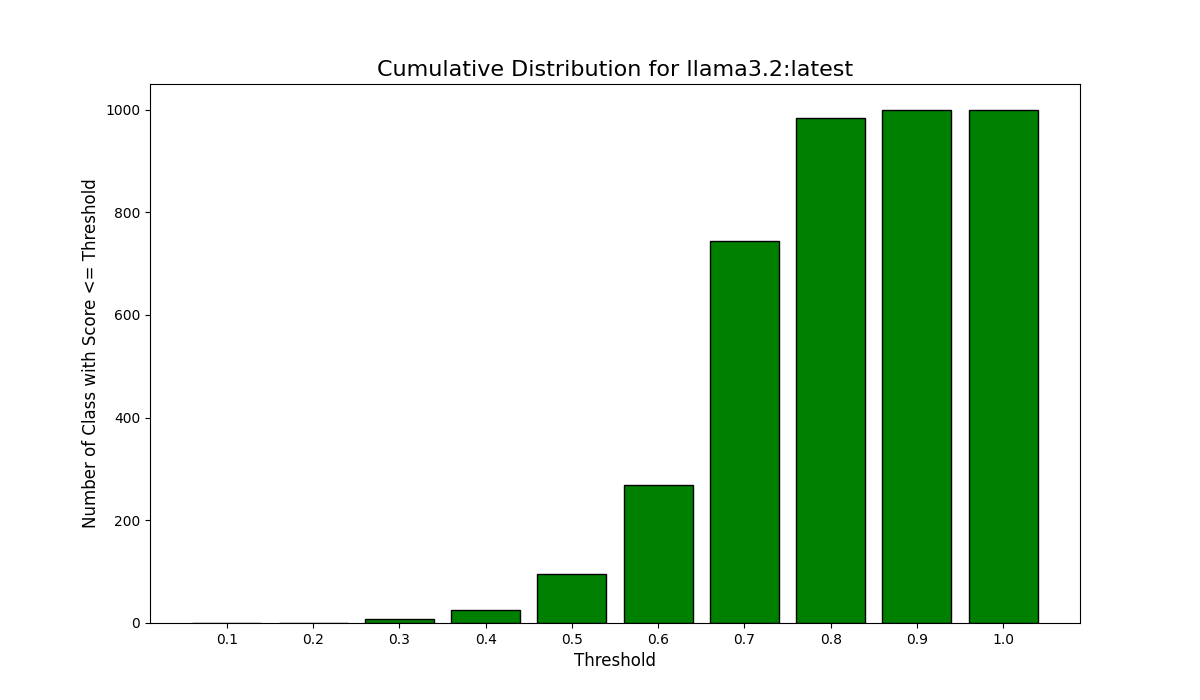
\includegraphics[width=0.55\textwidth]{img/CumulativeDistribution/CumulativeDistribution_llama3.2_latest.png} \\
\end{tabular}
\caption{Distribuzione Cumulativa dei CLIP Score per tutti i modelli}
\label{fig:cumulative_dist_all}
\end{figure}
In questi grafici, disegnamo le distribuzioni cumulative dove sull'asse y ci sono il numero di classi che sono minori o uguali del threshold mentre sull'asse x ci stanno i threshold possibili di score. Notiamo, quindi, che:
\begin{itemize}
    \item \textbf{Mistral:} ha delle classe che stanno anche sotto lo 0.2, quindi, puó capitare che ci siano allucinazioni.
    \item \textbf{Phi3:} sembra avere sicuramente una robustezza migliore alle allucinazioni, non dando peró un contributo significativo nella descrizione delle foto poiché dal grafico \ref{fig:dist_all} vediamo che i clipscore oscillano tra lo 0.4 e lo 0.5.
    \item \textbf{Gemma2:} ha una distribuzione cumulativa simile a quella del modello \textbf{Mistral}.
    \item \textbf{Llama3.2} simile a Mistral e Gemma2.
\end{itemize}
\textbf{Nota importante:} Phi3 mostra maggiore robustezza alle allucinazioni 
(poche classi sotto 0.3) ma genera descrizioni troppo generiche (concentrate 
0.4-0.5). Per applicazioni di generazione immagini, score nell'intervallo 
0.6-0.7 sono preferibili a 0.4-0.5, anche a costo di maggiore variabilità. 


\subsection{Tempi di Risposta}

\begin{figure}[H]
\centering
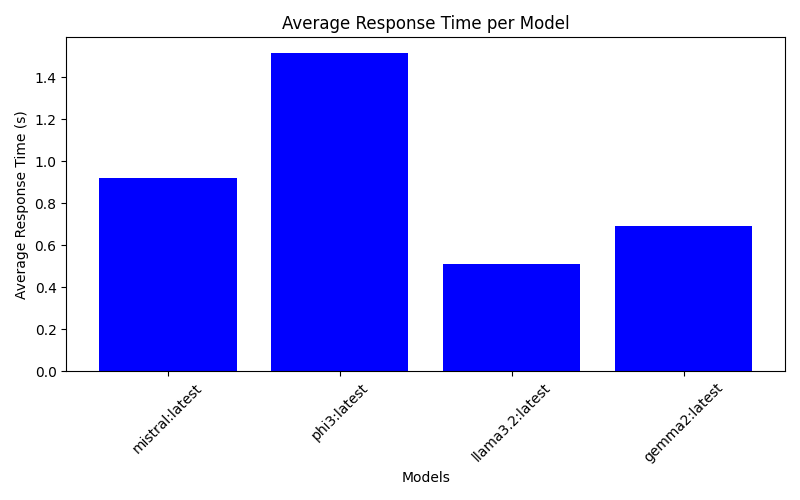
\includegraphics[width=0.7\textwidth]{img/avg_response_time.png}
\caption{Tempi medi di risposta per modello}
\label{fig:response_time}
\end{figure}
In questo grafico si descrive, invece, al variare del modello sull'asse x i tempi medi di risposta per una query.\
Quindi, dai tempi di risposta si capisce che:
\begin{itemize}
\item \textbf{Llama3.2} è il più veloce (circa 0.5s per prompt)
\item \textbf{Gemma2} e \textbf{Mistral} hanno tempi intermedi (0.7-0.9s)
\item \textbf{Phi3} è il più lento (circa 1.5s per prompt)
\end{itemize}

\subsection{Classi Sotto Soglia}

\begin{figure}[H]
\centering
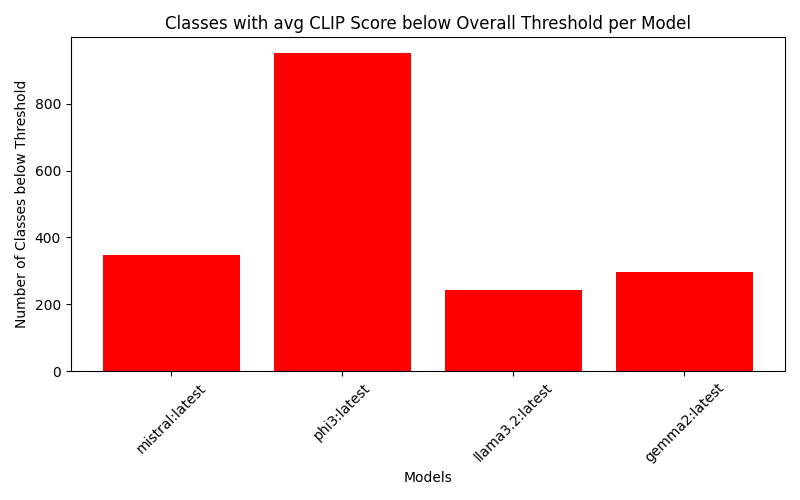
\includegraphics[width=0.7\textwidth]{img/classes_below_threshold.png}
\caption{Numero di classi con CLIP Score sotto la soglia media globale}
\label{fig:below_threshold}
\end{figure}

Come penultimo grafico, guarderemo un risultato che generalizza quello che abbiamo detto fino ad ora se calcoliamo la media globale del clipscore. Infatti vediamo che l'istogramma mostra un andamento di questo genere:\
\begin{itemize}
\item \textbf{Phi3} ha il maggior numero di classi sotto soglia (circa 950)
\item \textbf{Mistral} e \textbf{Gemma2} hanno circa 340 e 290 classi sotto soglia rispettivamente
\item \textbf{Llama3.2} ha il minor numero di classi sotto soglia (circa 240)
\end{itemize}\
\subsection{Media del ClipScore}
La seguente analisi rappresenta un esperimento che ho voluto fare per conto mio, realizzando alla fine che fosse fuori scopo.
Per completezza ho intenzione di pubblicare i risultati riguardo una classe specifica del nostro dataset.
\begin{figure}[H]
    \centering
    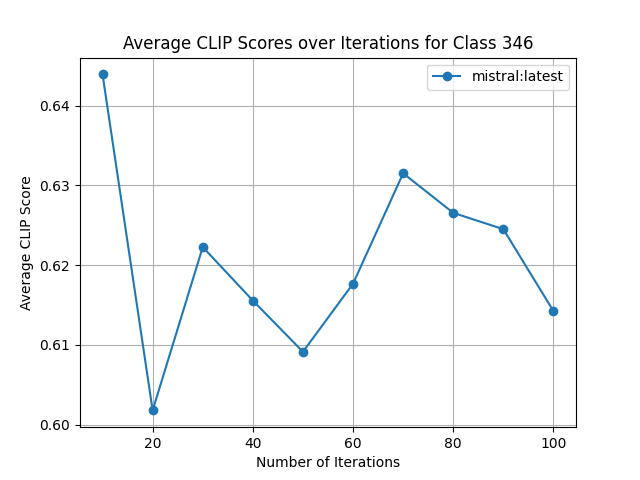
\includegraphics[width=0.75\linewidth]{img/wrong_result.png}
    \caption{Valore Medio del ClipScore al variare del numero di espasioni (Mistral)}
    \label{fig:wrong_result}
\end{figure}
L'obiettivo era quello di capire dopo quanti tentativi di espansione il ClipScore poteva stabilizzarsi. Cosa che é totalmente inutile visto che si tratta di una risposta di un modello su cui non abbiamo un controllo effettivo. 
\newpage

\section{Conclusioni}
I risultati dimostrano che la scelta del modello per la prompt expansion ha un impatto significativo sulla qualità delle descrizioni generate e, conseguentemente, sulla potenziale qualità delle immagini che potrebbero essere generate da un sistema text-to-image.
Dall'analisi complessiva emerge che:
\begin{itemize}
    \item \textbf{Llama3.2} risulta il modello più bilanciato, offrendo il miglior compromesso tra qualità delle espansioni (CLIP Score elevati) e velocità di elaborazione. È il modello raccomandato per applicazioni di prompt expansion.
    \item \textbf{Mistral} offre buone prestazioni in termini di qualità, con tempi di risposta accettabili, risultando una valida alternativa.
    \item \textbf{Gemma2} presenta prestazioni intermedie sia in termini di qualità che di velocità.
    \item \textbf{Phi3}, nonostante sia un modello compatto, mostra le prestazioni più deboli in questo specifico task di prompt expansion, sia in termini di CLIP Score che di tempo di elaborazione.
\end{itemize}


\subsection{Limitazioni e Considerazioni Tecniche}

Il modello CLIP utilizzato (openai/clip-vit-base-patch16) presenta una limitazione architetturale significativa: può processare al massimo \textbf{77 token} per ogni prompt testuale.
Infatti, quando un utente passa un prompt alla rete, un tokenizer scompone la frase in parole ed ad ognuna di essa gli associa un token, dopo di che questi token vengono processati tramite una Deep Neural Network, come detto prima, restituendo un vettore embedding.\\
Vengono utilizzati solo 77 token e quindi, nel nostro caso, il resto viene troncato, influenzando il risultato del embedding e, quindi, del ClipScore nel caso l'output sia troppo lungo.

\paragraph{Possibili Miglioramenti:}
Nel codice attuale non abbiamo controllo diretto sulla lunghezza dell'output dei modelli LLM. Tuttavia, potrebbero essere implementate le seguenti strategie:
\begin{itemize}
    \item \textbf{Controllo della temperatura:} Modificare il parametro di temperatura (che controlla il "livello di creatività" del modello) per ottenere output più concisi(Temperatura piú bassa). 
    \item \textbf{Prompt engineering:} Specificare esplicitamente nel prompt un limite di lunghezza (es. "generate a detailed description in maximum 50 words").
    \item \textbf{Post-processing:} Implementare un sistema di selezione delle frasi più rilevanti prima di passare il testo a CLIP, lo si puó fare tramite librerie NLP (come spacy).
    \item \textbf{Uso di modelli CLIP alternativi:} Esistono varianti di CLIP con limiti di token superiori che potrebbero essere esplorate in lavori futuri
    \item \textbf{Possibile Parallelizzazione:} di prompt expansion fatto dal modello.
\end{itemize}

\end{document}
